\chapter{Motivation}\label{chp:motivation}
Digitizing and vectorization is a time consuming and expensive process \cite{Worboys2003}.

In 2009, the Norwegian government made it statutory for all municipalities in Norway to have a digital zoning registers \cite{Kommunaltplanregister2009}. This has many benefits to society, both for the municipalities, the government, and the private sector. Benefits such as faster insights and sped up proceedings for building projects. 

In June 1st, 2017, 354 out of 426 municipalities are registered to have digital zoning registers. The law does however not force the municipalities to vectorize the zoning regulations in detail, only to have them scanned in a digital format such as Portable Document Format (PDF) with the bounding limits of the plan vectorized. The detailed vectorization is then another step that has to be done in order to fully utilize the data in more advanced use cases, such as in GIS. See \autoref{fig:examplezoning} for an example of a zoning regulation in PDF format.

For the municipalities, the digitalization and vectorization is a process that is often done by external contractors. In a project in Telemark and Vestfold, the cost was estimated to be around 3000NOK for each plan, where the whole project consisted of 100 plans \cite{Bo2009}. The cost savings in automating the vectorization of digitized zoning plans are thus economically significant. 

Since the zoning regulations has to follow strict quality standards, the acccuracy of the output from the DCNN also has to follow these standards. With many zoning regulations already digitized and vectorized, we potentially have a lot of validated, accurate data that can bee used to generate training data for the DCNN. This gives us a great oportunity to investigate the performance of DCNN for vectorization of scanned maps. 

There are a lot of approaches and network architectures that need to be examined and reviewed for this specific problem. This research will be the basis of the author's master thesis, where a practical implementation of the theory found in this research will be done. 


\begin{figure}[H]
	\centering
	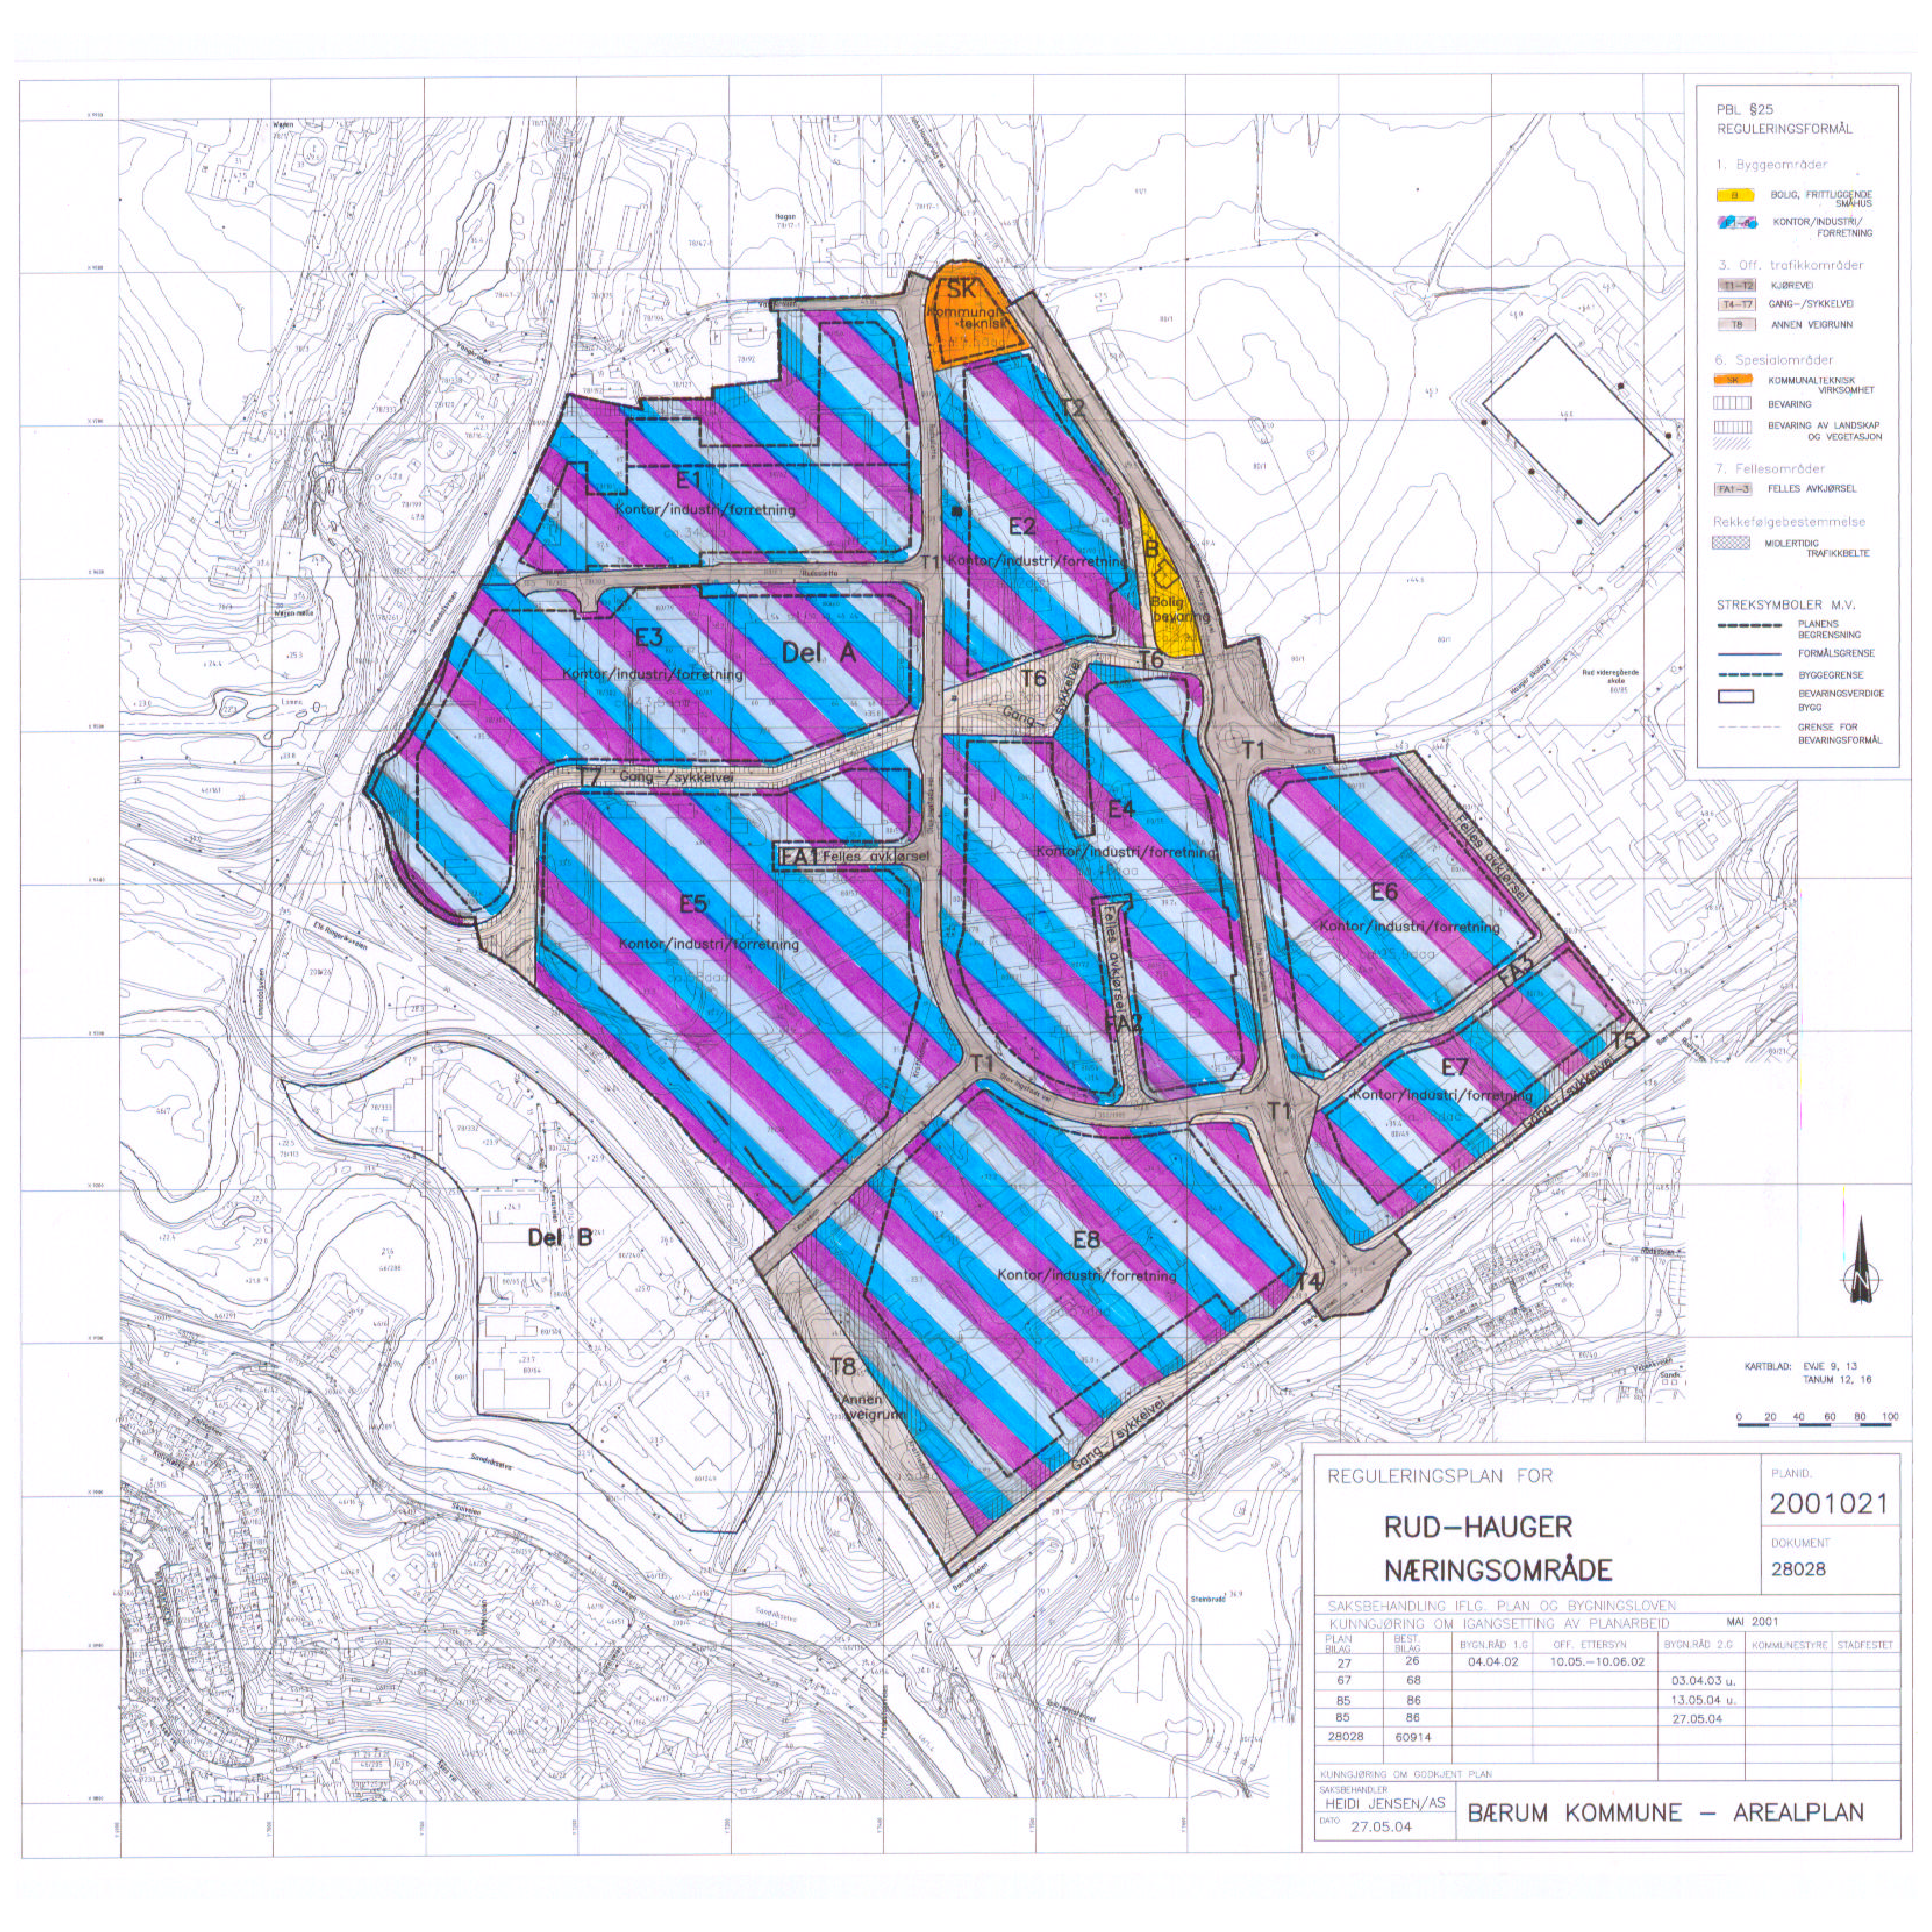
\includegraphics[width=0.8\linewidth]{fig/eksempel_plan.pdf}
	\caption{Scanned zoning regulation in PDF format from Bærum municipality. }
	\label{fig:examplezoning}
\end{figure}
